\documentclass[final]{siamltex}

\usepackage{graphicx}
\usepackage{subfigure}
\usepackage[colorlinks,unicode,linkcolor=black]{hyperref}
\usepackage{listings}
\lstset{
    language=C++,
    basicstyle=\small,
    columns=flexible,
    showstringspaces=false,
    numbers=left,
    numberstyle=\tiny,
    frame=lines
    }

\newcommand{\code}[1]{\lstinline|#1|}
\newcommand{\figref}[1]{Fig.~\ref{#1}}
\newcommand{\eqref}[1]{(\ref{#1})}

%
% mathematical commands
%
\newcommand {\de} {\mbox{d}}
\newcommand {\ii} {\mathop{i}}
\newcommand {\rem}[1]{}

\title{Programming OpenCL and CUDA:\\a Case Study Using Modern C++ Libraries}

\author{
Karsten Ahnert\thanks{Institut f\"ur Physik und Astronomie, Universit\"at Potsdam,
Karl-Liebknecht-Strasse 24/25, 14476 Potsdam-Golm, Germany ({\tt
karsten.ahnert@gmx.de}) }
\and Denis Demidov\thanks{
Kazan Branch of Joint Supercomputer Center,
Russian Academy of Sciences,
Lobachevsky st. 2/31, 420008 Kazan, Russia
({\tt ddemidov@ksu.ru}) }
\and Karl Rupp\thanks{Mathematics and Computer Science Division,
Argonne National Laboratory,
9700 South Cass Avenue, Argonne, IL 60439, USA
({\tt rupp@iue.tuwien.ac.at}) } }

\begin{document}

\maketitle

\begin{abstract}
    We present a comparison of several modern C++ libraries providing high-level interfaces
    for programming multi- and many-core architectures on top of OpenCL or CUDA.
    The comparison focuses on the solution of ordinary differential equations and is based on odeint,
    a framework for the solution of ordinary differential equations. Odeint is designed in a
    very flexible way and may be easily adapted for effective use of libraries such
    as VexCL, ViennaCL, or Thrust using OpenCL or CUDA technologies.
    We found that OpenCL and CUDA work equally well for problems
    of large sizes, while OpenCL has higher overhead for smaller problems.
    Furthermore, we show that modern high-level libraries allow to effectively
    use the computational resources of manycore GPUs or multicore CPUs without much
    knowledge of the underlying technologies.
\end{abstract}

\begin{keywords}
    GPGPU, OpenCL, CUDA, Modern C++ libraries, odeint, VexCL, ViennaCL, Thrust
\end{keywords}

\begin{AMS}
    34-04, 65-04, 65Y05, 65Y10, 68Q85, 97N80
\end{AMS}


%
% INTRODUCTION
%
\section{Introduction}

\pagestyle{myheadings}

\thispagestyle{plain}
\markboth{K.~AHNERT, D.~DEMIDOV, AND K.~RUPP}{PROGRAMMING CUDA AND OPENCL\ldots}


Recently, general purpose computing on graphics processing units (GPGPU) has
acquired considerable momentum in the scientific community. This is confirmed
both by increasing numbers of GPGPU-related publications and GPU based
supercomputers in the Top 500\footnote{ \href{ http://top500.org }{
http://top500.org }} list. Major programming frameworks are NVIDIA CUDA and
OpenCL.  The former is a proprietary parallel computing architecture developed
by NVIDIA for general purpose computing on NVIDIA graphics adapters, and the
latter is an open, royalty-free standard for cross-platform, parallel
programming of modern processors maintained by the Khronos group. By nature,
the two frameworks have their distinctive pros and cons. CUDA has a more mature
programming environment with a larger set of scientific libraries, but is
available on NVIDIA hardware only. OpenCL is supported on wide range of hardware,
but its native API requires a much larger amount of boilerplate code from a
developer.

Both technologies are able to provide scientists with the vast computational
resources of modern GPUs at the price of a steep learning curve.
Programmers need to familiarize
themselves with a new programming language and, more importantly, with a
new programming paradigm. However, the entry barrier may be lowered with the help of
specialized libraries. The CUDA Toolkit includes several such libraries (BLAS
implementations, Fast Fourier Transform, Thrust and others). OpenCL lacks
standard libraries, but there are a number of third-party projects aimed at
developing both CUDA and OpenCL programs.

This paper presents a comparison of several modern C++ libraries aimed
at ease of GPGPU development. We look at both convenience and
performance of the libraries under consideration in the context of
solving ordinary differential equations.  The comparison is based on
odeint, a modern C++ library for solution of ordinary differential equations (ODEs) that has been recently
included into the Boost libraries\footnote{ \href{ http://boost.org }
  { http://boost.org } }.  The GPGPU libraries considered in this work
are Thrust, VexCL, and ViennaCL:

% [KR]: We need to define the scope of this work. We are investigating ODEs
% only, which we have to clarify.  There is a lot of GPGPU for dense linear
% algebra, sparse solvers, and molecular dynamics approaches. We don't consider
% any of these.

% [DD]: Is `the context of solving ordinary differential equations` not enough
% for this purpose? Or should we explicitly state that we are not intersted in
% the topics you mentioned?

\begin{description}
    \item[Odeint] is a modern C++ library \footnote{ \href{ http://odeint.com }{
        http://odeint.com } } for solving ODEs numerically \cite{OdeintRef1, OdeintRef2}.
        It is developed in a generic
        way using template metaprogramming techniques, which leads to extraordinary high
        flexibility at utmost performance. The numerical algorithms are
        implemented independently of the underlying arithmetics. This results
        in a broad applicability of the library, especially in non-standard
        environments.  For example, odeint supports matrix types, arbitrary
        precision arithmetics, and can be easily adopted to use either CUDA or
        OpenCL frameworks.  Odeint is used in this work as a framework for the
        comparison of other libraries.
    \item[Thrust] is a parallel algorithms library\footnote{ \href{
        http://thrust.github.com }{ http://thrust.github.com }} which resembles
        the C++ Standard Template Library \cite{ThrustRef}.  Thrust's
        high-level interface greatly enhances developer productivity while
        enabling performance portability between GPUs and multicore CPUs.
        Thrust is distributed with the NVIDIA CUDA Toolkit since version 4.1.
    \item[VexCL] is vector expression template
        library\footnote{ \href{ https://github.com/ddemidov/vexcl }{
        https://github.com/ddemidov/vexcl }} for OpenCL \cite{VexCLRef}. It has
        been created for ease of OpenCL development with C++.  VexCL strives to
        reduce the amount of boilerplate code needed to develop OpenCL
        applications. The library provides a convenient and intuitive notation
        for vector arithmetic, reduction, and sparse matrix-vector
        multiplication.  Multi-device and even multi-platform computations are
        supported.
    \item[ViennaCL] (The Vienna Computing Library) is a scientific computing
        library\footnote{ \href{ http://viennacl.sourceforge.net }{
        http://viennacl.sourceforge.net }} written in C++ and based on OpenCL
        \cite{ViennaCLRef}. Its interface is compatible with
        Boost.uBLAS\footnote{ \href{ http://www.boost.org/libs/numeric/ublas }
        { http://www.boost.org/libs/numeric/ublas } }
        and allows for simple, high-level access to the vast
        computing resources available on parallel architectures such as GPUs.
        The library's primary focus is on common linear algebra operations (BLAS
        levels 1, 2 and 3) and the solution of large systems of equations by
        means of iterative methods with optional preconditioner.
\end{description}

CUDA and OpenCL differ in their handling of compute kernels compilation. In
NVIDIA's framework the compute kernels are compiled to PTX code together with
the host program. The PTX is a pseudo-assembler language which is compiled at
runtime for the specific NVIDIA device the kernel is launched on. Since PTX is already
very low-level, this just-in-time kernel compilation has low overhead. In
OpenCL the compute kernels are compiled at runtime from higher-level C-like sources.
This adds an overhead which is particularly noticeable for smaller sized
problems. A pre-compilation to some low-level pseudo-code as in CUDA is not feasible in
OpenCL because of hardware agnosticism by design.

The approach taken for the generation and compilation of the compute kernels is one of the
main differences between the OpenCL libraries we considered.
ViennaCL uses a set of predefined kernels, which functionally overlaps with BLAS level
1 routines for vector operations.
These kernels are compiled in batch at the program start to allow
for faster initialization. However, due to this design decision each vector
expression may result in the launch of more than one kernel.  On the other hand,
VexCL generates and compiles an OpenCL program with a single kernel for each
vector expression it encounters.  This leads to potentially higher
initialization overhead, but should prove to be more effective in the long
runs. It should be noted that because of the main focus of ViennaCL being on iterative
solvers for large sparse systems of equations, where complex vector
expressions are rare, predefined kernels are favorable in such a setting.
The implications of these two distinct design decisions in VexCL and ViennaCL will be further addressed in the discussion of the results.

The other difference between CUDA and OpenCL is that CUDA supports a subset of the
C++ language in compute kernels, while OpenCL kernels are written in subset of
C99. Therefore, CUDA programmers may use template metaprogramming techniques
which may lead to more efficient and compact code. The native OpenCL API does not
provide such a feature, but the drawback is balanced by the ability of
kernel source generation during runtime. Modern C++ libraries such as those considered in
this work successfully use this approach and hide gory details from their
users.




%
% ADAPTING ODEINT
%
\section{Adapting odeint} \label{sec:adapting-odeint}

Ordinary differential equations play a major role in many scientific
disciplines. They occur naturally in the context of mechanical
systems, like granular and molecular dynamics. In fact, the Newtonian
and Hamiltonian mechanics are formulated as ODEs.
Many other applications can be found in such diverse
fields as biology and neuroscience, chemistry, and social sciences. % [KR] Citations required here!
Furthermore, ODEs are also encountered in the context of the numerical solution of nonstationary partial
differential equations (PDEs), where they occur after the discretization of the spatial coordinates. % [KR] This is probably the most common case

Odeint usually solves % [KR]: 'usually solves' is a bit too fuzzy. Does it support other types (implicit ODEs, higher-order ODEs)? If yes, we should state that here.  It is advisable to define the scope properly in a SIAM Journal.
the initial value problem (IVP) of ordinary differential equations.
\begin{equation}
\frac{\de x}{\de t } = \dot{x} = f(x , t), \quad \quad x(0) =
x_0.
\label{eq:ode}
\end{equation}
Here, $x$ is the dependent variable and is usually a vector of real or complex values.
$t$ is the independent variable. We will refer to $t$ as the time throughout the article and
denote the time derivative with $\de x / \de t = \dot{x}$. $f(x,t)$ is
the system function and defines the ODE.

Numerous methods for solving ODEs exist \cite{HairerSolvingODEI,
  HairerSolvingODEII, HairerGeometricNumericalIntegration2006}, % [KR]: I would prefer a more diverse set of authors here (not just Hairer)
which are usually categorized in the field of numerical analysis.
Odeint
implements the most prominent of these methods, for example the
classical Runge-Kutta methods and Runge-Kutta-Fehlberg methods,
multistep methods (Adams-Bashforth-Moulton), symplectic
Runge-Kutta-Nystr\"om methods, and implicit methods (Rosenbrock and
implicit Euler). All of these methods work iteratively, starting
from a given initial value $x(t_0)$ to calculate the next value
$x(t+\Delta t)$.
$\Delta t$ is the step size and many be chosen either statically or adaptively.
For reference, we note that the simplest method is the explicit Euler scheme
\begin{equation}
x\left(t+\Delta t\right) := x(t) + \Delta t \; f(x(t),t) .
\label{eq:euler}
\end{equation}
Its global accuracy is of first order, but the scheme is usually not used for real applications because of stability issues.


One main feature of odeint is the decoupling of the specific algorithm
for solving the ODE from the underlying arithmetic operations. This
is achieved by a combination of a state type, an algebra, and
operations. The state type represents the state of the ODE being
solved and is usually a vector type like \code{std::vector<>},
\code{std::array<>}, or a vector residing on a GPU. The algebra is
responsible for iterating through all elements of the state whereas
the operations are responsible for the elementary operations.

To see how the explicit Euler method \eqref{eq:euler} is translated to
code in odeint, we briefly discuss its implementation:
\begin{lstlisting}
template< class State, class Algebra, class Operations >
class euler {
    // ...
    template< class Ode >
    void do_step(Ode ode, State &x, time_type t, time_type dt) {
        ode(x, m_dxdt, dt);
        Algebra::for_each3( x, x, m_dxdt, Operations::scale_sum2(1.0, dt) );
    }
};
\end{lstlisting}
The state type, the algebra, and the operations enter the stepper  % [KR]: It is not yet defined what a 'stepper'...
as template parameter, hence they are exchangeable. The function object
\code{ode} represents the ODE and must be provided by the user. It calculates
the right hand side $f(x,t)$ of \eqref{eq:ode} and stores the result in
\code{m_dxdt}. The call of \code{for_each3} iterates three vectors and    % [KR]: This is a bit confusing. What does 'iterate three vectors' mean in this context? It is not obvious how the for_each3-scale_sum2-call equals x(t) + \Delta t \; f(x(t),t) .
applies on each element \code{scale_sum2}. The operation is performed
in-place, meaning that $x$ is updated to the new value.
In the code-snippet above, the call to \code{for_each3} is thus equivalent to the vector operation
\begin{lstlisting}
 x = 1.0 * x + dt * m_dxdt
\end{lstlisting}
which is just \eqref{eq:euler}, since \code{m_dxdt} holds the values of $f(x(t), t)$.
The main reason for the separation of algebra and operations is that all arithmetic calculations and
iterations are completely encapsulated into the algebra and the
operations which must be provided by the user. Note, that algebra and
the operations must be chosen such that they interact correctly with
the state type.

% [KA]: Maybe the paragraph above explains the functioning a bit better.
% The paragraph is not finished and
% it requires to put the paragraphs about ODEs in front of this paragraph.

% [DD]: I like it better than the paragraph below. That I took from odeint
% documentation and it feels out of context here. May be we should omit it.

% [KR]: The paragraph below also appears to be way too much implementation
%       It is not really relevant for what follows, so I prefer to omit it.
%       I commented it in the meanwhile.

% Odeint provides a set of predefined algebras, which includes:
% \begin{remunerate}
% \item \code{range_algebra}: default algebra which works on Boost.Ranges;
% \item \code{array_algebra}: specialized algebra for \code{boost::array};
% \item \code{fusion_algebra}: algebra for compile-time sequences like
%   \code{boost::fusion::vector}, \code{std::tuple}, etc.;
% \item \code{vector_space_algebra}: algebra for vector space types that
%   provide overloaded arithmetic operators for elementwise operations.
% \end{remunerate}
% Each of these algebras is a class consisting of \code{for_each1},
% \dots, \code{for_eachN} methods. For example the \code{for_each3}
% method in the \code{range_algebra} is similar to
% \begin{lstlisting}
% struct range_algebra {
%     // ...
%     template< class R1, class R2, class Op >
%     void for_each2(R1 &r1, R2 &r2, Op op) {
%         auto it1 = boost::begin(r1);
%         auto it2 = boost::begin(r2);
%         while(it1 != boost::end(r1)) op( *it1++, *it2++ );
%     }
%     // ...
% };
% \end{lstlisting}
% The operations are represented by a struct with public member classes defining the
% operations which are used by the algebras. There is only one default
% operations class implementation in odeint
% \begin{lstlisting}
% struct default_algebra {
%     // ...
%     template< class Fac1, class Fac2 >
%     struct scale_sum2 {
%         Fac1 m_fac1;
%         Fac2 m_fac2;
%         scale_sum2( Fac1 fac1, Fac2 fac2 ) : m_fac1(fac1), m_fac2(fac2) { }
%         template< class S1, class S2, class S3 >
%         void operator()( S1 &s1, const S2 &s2, const S3 &s3 ) const {
%             s1 = m_fac1 * s2 + m_fac2 * s3;
%         }
%     };
%     // ...
% };
% \end{lstlisting}

% [KR]: Rephrased the following paragraph a bit to account for the removal of the previous paragraph
Many libraries for vector and matrix types provide expression
templates \cite{Veldhuizen:ExpressionTemplates, Veldhuizen:Techniques,
Vandevoorde:CppTemplates} for the elementary operations using operator overload
convenience.
Such libraries do not need to define their own algebra,
but can instead be used with a default algebra
and a default operation set included in odeint,
which simply call the operations directly on the matrix or vector type.
In this case only the resizing mechanism of odeint has to be adapted for the new types.

We describe the adaptation of odeint for the GPGPU libraries under consideration
in the following. The adaptions are now part of odeint, thus native support
for these libraries is available.
Implementation details such the resizing of vectors is accomplished in a straight-forward manner
and not further addressed for the sake of conciseness.
% [KR]: I don't think that we need to justify the discussion with the next sentence. The paper is just about this topic :-)
%However, providing
%adaptation examples serves our goal of comparing convenience of the
%libraries interfaces.

To adapt Thrust to odeint we need to provide both an algebra and
operations. The algebra needs to define the \code{for_each} family of
algorithms. All of these operations follow the same pattern,
so we consider \code{for_each3} only:
\begin{lstlisting}
struct thrust_algebra {
    template<class StateType1, class StateType2, class StateType3, class Oper>
    static void for_each3(StateType1 &s1, StateType2 &s2, StateType3 &s3, Oper op)
    {
        thrust::for_each(
                thrust::make_zip_iterator( thrust::make_tuple(
                    boost::begin(s1), boost::begin(s2), boost::begin(s3) ) ),
                thrust::make_zip_iterator( thrust::make_tuple(
                    boost::end(s1), boost::end(s2), boost::end(s3) ) ),
                op);
    }
};
\end{lstlisting}
Here, \code{thrust::make_zip_iterator} is used in combination with \code{make_tuple}
to pack several device vector iterators into a single iterable sequence.
The sequence is then processed by the \code{thrust::for_each} algorithm, applying the function object
\code{op} to each entry.

The operations called via the function object \code{op} defined in \code{thrust_operations}
and are actually function objects executed on the respective CUDA device:
\begin{lstlisting}
struct thrust_operations {
    template<class Fac1 = double, class Fac2 = Fac1>
    struct scale_sum2 {
        const Fac1 m_alpha1;
        const Fac2 m_alpha2;

        scale_sum3(const Fac1 alpha1, const Fac2 alpha2)
            : m_alpha1(alpha1), m_alpha2(alpha2) { }

        template< class Tuple >
        __host__ __device__ void operator()( Tuple t ) const {
            thrust::get<0>(t) = m_alpha1 * thrust::get<1>(t)
                               + m_alpha2 * thrust::get<2>(t);
        }
    };
\end{lstlisting}
The device function object uses \code{thrust::get<>} functions to unpack the zip iterator into separate values.
This approach is heavily used with Thrust and allows to process several vectors
in single efficient sweep.
% [KR] The following sentence refers to an implementation detail and is not of importance for the performance, thus I commented it.
%Adaptation of resizing operations is trivial and is
%omitted here for the sake of conciseness.


Both VexCL and ViennaCL provide convenient expression templates that
may be directly used with odeint's \code{vector_space_algebra} and
\code{default_operations}. This combination proved to be
effective with VexCL, where each expression results in a single
kernel. For ViennaCL, however, default operations involving more than two
terms result in multiple kernel launches.  Moreover, temporary vectors
are allocated and deallocated for each of such composite operations, resulting in a dramatic decrease of performance.
To address such problems, ViennaCL provides a kernel generator \cite{tillet:kernel-generator}, which is able to generate
specialized operations for ViennaCL. These use a custom kernel
generation mechanism provided by the library.  For example,
\code{scale_sum2} operation is defined as:
\begin{lstlisting}
struct viennacl_operations {
    // ...
    template<class Fac1 = double, class Fac2 = Fac1>
    struct scale_sum2 {
        // ...
        template<class T1, class T2, class T3>
        void operator()( viennacl::vector<T1> &v1,
                const viennacl::vector<T2> &v2,
                const viennacl::vector<T3> &v3) const
        {
            using namespace viennacl;

            // instantiate symbolic types:
            static generator::symbolic_vector    <0, T1>   sym_v1;
            static generator::symbolic_vector    <1, T2>   sym_v2;
            static generator::symbolic_vector    <2, T3>   sym_v3;
            static generator::cpu_symbolic_scalar<3, Fac1> sym_a1;
            static generator::cpu_symbolic_scalar<4, Fac2> sym_a2;

            // run the kernel generation at first call of this function:
            static generator::custom_operation op(
                    sym_v1 = sym_a1 * sym_v2 + sym_a2 * sym_v3,
                    "scale_sum2");

            // launch the kernel:
            ocl::enqueue( op(v1, v2, v3, m_alpha1, m_alpha2) );
        }
    };
    // ...
};
\end{lstlisting} % [KR]: The const_cast<> was necessary due to an oversight of 'const' in the operator overloads. This is now fixed.
Here, a custom OpenCL kernel is automatically generated from symbolic vector expression
in the first call of the \code{operator()} and then reused for all subsequent calls.

\section{Numerical Experiments}

As shown in the previous section, all three GPGPU libraries considered in our comparison
could be adapted to odeint without getting in contact with low-level CUDA or OpenCL code.
The purpose of this section is to evaluate the performance of the GPGPU libraries and whether there is a price to pay for the high-level interface.

%% [KR]: This paragraph is mostly a duplication of what has been said in the introduction...
Typical use cases for solving ODEs on GPUs are large systems of
coupled ODEs which occur as discretizations of PDEs, or in ODEs
defined on lattices or graphs. Another use case are parameter studies,
where one wants to study the dependence of an ODE on some
parameters. Here, one creates one large ODE which consists of many
small uncoupled ODEs, each with a different parameter set. This one
large system is then solved at once, hence all small ODEs are solved
simultaneously.

In this section we will show four examples and study their
performance. Two examples are of the first type, namely a
one-dimensional lattice of simple phase oscillators and a
two-dimensional Hamiltonian lattice. The other two examples are
parameter studies.




%
% DAMPED OSCILLATOR
%
\subsection{Damped Harmonic Oscillator Ensemble}

The first example is a set of damped driven oscillators as described by the system
\begin{equation} \label{eq:dampedsystem}
    \dot{x} =  \varepsilon x + \omega y , \quad \quad
    \dot{y} =  \varepsilon y - \omega x
\end{equation}
with $\varepsilon = \varepsilon_0 + \varepsilon_a \cos \left( \omega_d    % [KR]: We should give \varepsilon a name here. Is it a 'damping function'?
t \right)$. $\omega$ is the natural frequency of the oscillator and
$\varepsilon$ is the time dependent damping constant.  Note that this form is
not the classical form $\ii \dot{\Psi} = \omega \Psi + \ii \varepsilon \Psi$ of a damped oscillator,
but can be derived easily by setting $\Psi = x + \ii y$.


The Thrust version of the system functor for the damped harmonic oscillator
ensemble example is presented below. The functor holds model parameters and
provides \code{operator()} with a signature required by the odeint library. The
state type is represented by \code{thrust::device_vector<double>}:
\begin{lstlisting}
typedef thrust::device_vector<double> state_type;

struct oscillator {
    size_t N;
    double omega, amp, offset, omega_d;

    oscillator(size_t N, double omega, double amp, double offset, double omega_d)
        : N(N), omega(omega), amp(amp), offset(offset), omega_d(omega_d) { }

    void operator()(const state_type &x, state_type &dxdt, double t) const;
};
\end{lstlisting}
The $X$ and $Y$ components of the state are held in the first and second halves of the
vector.  \code{operator()} uses the standard technique of
packing the state components into a zip iterator and passes the composite
sequence to the \code{thrust::for_each} algorithm together with the provided device
functor:
\begin{lstlisting}[firstnumber=12]
struct oscillator_functor;

void oscillator::operator()(const state_type &x, state_type &dxdt, double t) const {
    double eps = offset + amp * cos(omega_d * t);
    thrust::for_each(
        thrust::make_zip_iterator(
            thrust::make_tuple( boost::begin(x), boost::begin(x) + N,
                                boost::begin(dxdt), boost::begin(dxdt) + N ) ),
        thrust::make_zip_iterator(
            thrust::make_tuple( boost::begin(x) + N, boost::end(x),
                                boost::begin(dxdt) + N, boost::end(dxdt) ) ),
        oscillator_functor(omega, eps) );
}
\end{lstlisting}
The device functor unpacks the individual components and applies the required
operations to the derivative part, essentially leading to a one-to-one translation of \eqref{eq:dampedsystem} into code:
\begin{lstlisting}[firstnumber=last]
struct oscillator_functor {
    double eps, omega;

    oscillator_functor(double omega, double eps) : omega(omega), eps(eps) {}

    template< class T >
    __host__ __device__ void operator()(T t) const {
        double x = thrust::get< 0 >( t );
        double y = thrust::get< 1 >( t );
        thrust::get<2>(t) = eps * x + omega * y;
        thrust::get<3>(t) = eps * y - omega * x;
    }
};
\end{lstlisting}


The system functor for the VexCL version of the damped harmonic oscillator
example is much simpler than the Thrust variant because VexCL supports a rich
set of vector expressions. The state is represented by the
\code{vex::multivector<double,2>} type, which holds two instances of
\code{vex::vector<double>} and transparently dispatches all operations to the
underlying components. The code for \code{operator()} body practically
coincides with the problem statement \eqref{eq:dampedsystem}:
\begin{lstlisting}
typedef vex::vector<double> vector_type;
typedef vex::multivector<double, 2> state_type;

struct oscillator {
    double omega, amp, offset, omega_d;

    oscillator(double omega, double amp, double offset, double omega_d)
        : omega(omega), amp(amp), offset(offset), omega_d(omega_d) { }

    void operator()(const state_type &x, state_type &dxdt, double t) const {
        double eps = offset + amp * cos(omega_d * t);
        dxdt(0) = eps * x(0) + omega * x(1);
        dxdt(1) = eps * x(1) - omega * x(0);
    }
};
\end{lstlisting}


However, the drawback of this variant is that it leads
to two kernel launches (one per each vector assignment), resulting in
suboptimal performance. A direct use of multivector arithmetic
operations is not possible due to mixed components in the right hand side expressions.
The additional kernel launch can be eliminated in VexCL by assigning a tuple of expressions to a multivector.
The required notation is only slightly more cumbersome than the above variant:
\begin{lstlisting}[firstnumber=11]
        double eps = offset + amp * cos(omega_d * t);
        dxdt = std::make_tuple(     eps * x(0) + omega * x(1),
                                    eps * x(1) - omega * x(0)   );
\end{lstlisting}

For the ViennaCL version of the damped harmonic oscillator ensemble example a
\code{boost::fusion::vector} is used to pack the coordinate components of the state vector into a
single type. Individual components are instances of the
\code{viennacl::vector<double>} type.

ViennaCL, as well as VexCL, supports expression templates for a limited set of    %[KR]: Denis, isn't VexCL supporting arbitrary vector operations? Are you referring with 'as well as VexCL' to expression templates only?
vector operations (closely corresponding to Level 1 BLAS routines).
Thus, one can use similar code as for the first version of VexCL presented above,
yet obtain suboptimal performance due to two kernel launches per step.
Similar to VexCL, ViennaCL offers a mechanism to get rid of the second kernel launch
with the help of the ViennaCL kernel generator interface, which supports kernels with single and multipleoperations.
Here, OpenCL kernels are generated from symbolic expressions involving explicit symbolic types,
which is a bit more cumbersome than with VexCL. In particular, the constructor
for the oscillator implementation usnig ViennaCL is given by
%\begin{lstlisting}
%typedef viennacl::vector<double> vector_type;
%typedef fusion::vector<vector_type, vector_type> state_type;
%
%struct oscillator {
%    double omega, amp, offset, omega_d;
%
%    viennacl::generator::symbolic_vector<0, double> sym_dx;
%    viennacl::generator::symbolic_vector<1, double> sym_dy;
%    viennacl::generator::symbolic_vector<2, double> sym_x;
%    viennacl::generator::symbolic_vector<3, double> sym_y;
%    viennacl::generator::cpu_symbolic_scalar<4, double> sym_eps;
%    viennacl::generator::cpu_symbolic_scalar<5, double> sym_omega;
%    viennacl::generator::custom_operation op;
%
% [KR] Stripped this snippet, because symbolic types have been used in Section 2 already.
\begin{lstlisting}
    oscillator(double omega, double amp, double offset, double omega_d)
        : omega(omega), amp(amp), offset(offset), omega_d(omega_d),
          op(sym_dx = sym_eps * sym_x + sym_omega * sym_y,
             sym_dy = sym_eps * sym_y - sym_omega * sym_x,
             "oscillator")
    { }
\end{lstlisting}
%
%    void operator()( const state_type &x, state_type &dxdt, double t );
%};
%\end{lstlisting}
The symbolic types \code{sym_dx}, \code{sym_dy}, etc.~are instantiated in the same way
as in the code snippet given at the end of Sec.~\ref{sec:adapting-odeint}.
Even though more boilerplate code is required, the resulting expression
carries explicit information of whether two terminals represent the same vector
instance. This in principle allows generation of more effective code. The
\code{operator()} unpacks the \code{fusion::vector} container and launches
the generated kernel:
\begin{lstlisting}
void oscillator::operator()( const state_type &x, state_type &dxdt, double t ) {
    vector_type &X  = const_cast<vector_type&>( fusion::at_c<0>(x) );
    vector_type &Y  = const_cast<vector_type&>( fusion::at_c<1>(x) );
    vector_type &dX = fusion::at_c<0>(dxdt);
    vector_type &dY = fusion::at_c<1>(dxdt);

    double eps = offset + amp * cos(omega_d * t);
    viennacl::ocl::enqueue( op(dX, dY, X, Y, eps, omega) );
}
\end{lstlisting}




%
% PHASE OSCILLATORS
%
\subsection{Chain of Coupled Phase Oscillators}

As a second example we consider a chain of coupled phase
oscillators. A phase oscillator describes the dynamics of an
autonomous oscillator \cite{PhaseOscillator}. Its evolution is
governed by the phase $\varphi$, which is a $2\pi$ -eriodic variable growing linearly
in time, i.e.~$\dot{\varphi} = \omega$, where $\omega$ is the phase
velocity. The amplitude of the oscillator does not occur in this
equation, so an interesting behavior can only be observed if many
of such oscillators are coupled. In fact, such a system can be used to
study such divergent phenomena as synchronization, wave and pattern
formation, phase chaos, or oscillation death
\cite{Synchronization-Pikovsky,Kuramoto-84}. It is a prominent example
of an emergent system where the coupled system shows a more complex
behavior than its constitutes.


The concrete example we analyze here is a chain of nearest-neighbor
coupled phase oscillators:
\begin{equation} \label{eq:phasesystem}
    \dot{\varphi}_i = \omega_i + \sin( \varphi_{i+1} - \varphi_i) + \sin( \varphi_i
    - \varphi_{i-1}).
\end{equation}
The index $i$ denotes here the $i$-th phase in the chain. Note, that
the phase velocity is different for each oscillator.

The Thrust version for the coupled phase oscillator chain looks very similar to
the damped oscillator example. Again, a zip iterator is used to pack the required
components and to process the resulting sequence with single sweep of the
\code{for_each} algorithm. The only difference here is that values of
neighboring vector elements are needed. In order to provide the values, we use Thrust's
permutation iterator, so that \code{operator()} of the system function object becomes
\begin{lstlisting}
thrust::for_each(
    thrust::make_zip_iterator(
        thrust::make_tuple(
            x.begin(),
            thrust::make_permutation_iterator( x.begin(), prev.begin() ),
            thrust::make_permutation_iterator( x.begin(), next.begin() ),
            omega.begin(),
            dxdt.begin() ) ),
    thrust::make_zip_iterator(
        thrust::make_tuple(
            x.end(),
            thrust::make_permutation_iterator( x.begin(), prev.end() ),
            thrust::make_permutation_iterator( x.begin(), next.end() ),
            omega.end(),
            dxdt.end() ) ),
    sys_functor()
    );
\end{lstlisting}
\code{prev} and \code{next} are vectors of type
\code{thrust::device_vector<size_t>} and hold the indices to the left and right vector
elements.
% [KR]: I consider the following an implementation detail, hence commented:
%and initialized as
%\begin{lstlisting}
%thrust::counting_iterator<size_t> c(0);
%thrust::copy(c, c + N - 1, prev.begin() + 1);
%prev[0] = 0;     // prev = { 0, 0, 1, 2, 3, ..., N-1 }
%thrust::copy(c + 1, c + N, next.begin());
%next[N-1] = N-1; // next = { 1, 2, 3, ..., N-1, N-1 }
%\end{lstlisting}

The VexCL version of the example is the most
concise variant since VexCL provides native support for the user-defined
stencils operations. The sum of sines in \eqref{eq:phasesystem} is encoded
using the \code{vex::StencilOperator<>} class template.  Template parameters
are the body string for the generated OpenCL function encoding required
operation, width and center point of the stencil, and its return type. Once the
stencil operator is defined, the functor's \code{operator()} is implemented
with a single line of code:
\begin{lstlisting}
typedef vex::vector<double> state_type;
extern const char oscillator_body[] = "return sin(X[-1] - X[0]) + sin(X[0] - X[1]);";

struct phase_oscillators {
    const state_type &omega;
    vex::StencilOperator< double, 3, 1, oscillator_body > S;
    phase_oscillators(const state_type &omega)
        : omega(omega), S(omega.queue_list()) { }
    void operator()(const state_type &x, state_type &dxdt, double t) const {
        dxdt = omega + S(x);
    }
};
\end{lstlisting}


ViennaCL, being oriented at iterative solution of large systems of equations,
does not provide stencil operations required for the problem at hand, so we had
to fallback to the use of a hand-coded OpenCL kernel, which is omitted for reasons of brevity.
%\begin{lstlisting}
%static const char phase_oscillator_source[] =
%    "#pragma OPENCL EXTENSION cl_khr_fp64: enable\n"
%    "kernel void oscillator(\n"
%    "        uint n,\n"
%    "        global double *dx,\n"
%    "        global const double *x,\n"
%    "        global const double *omega\n"
%    "        )\n"
%    "{\n"
%    "    for(uint i = get_global_id(0); i < n; i += get_global_size(0)) {\n"
%    "        double X0 = x[i];\n"
%    "        double Xl = i > 0 ? x[i - 1] : X0;\n"
%    "        double Xr = i + 1 < n ? x[i + 1] : X0;\n"
%    "        dx[i] = omega[i] + sin(Xl - X0) + sin(X0 - Xr);\n"
%    "    }\n"
%    "}\n";
%\end{lstlisting}
Even though a custom OpenCL kernel needs to be used for this example,
ViennaCL provides convenient mechanisms for the compilation and launch of custom
kernels, avoiding tedious interactions with the low-level OpenCL API.
As a consequence, the performance of ViennaCL for this example is comparable to hand-tuned code.
The actual implementation of the \code{phase_oscillators} class consequently consists
of the compilation of the kernel residing in a string object \code{phase_oscillator_source} in the constructor,
and the launch of the respective kernel in \code{operator()}:
\begin{lstlisting}
typedef viennacl::vector<double> state_type;

struct phase_oscillators {
    const state_type &omega;
    sys_func(const state_type &omega) : omega(omega) {
        viennacl::ocl::current_context().add_program(phase_oscillator_source,
            "oscillator_program").add_kernel("oscillator");
    }
    void operator()(const state_type &x, state_type &dxdt, double t) const {
        viennacl::ocl::kernel &step = viennacl::ocl::current_context().get_program(
            "oscillator_program").get_kernel("oscillator");
        viennacl::ocl::enqueue( step(static_cast<cl_uint>(x.size()), dxdt, x, omega) );
    }
};
\end{lstlisting}








%
% DISORDERED LATTICES
%
\subsection{Disordered Hamiltonian Lattice}


Another example for our performance and usage study is a strongly
nonlinear disordered Hamiltonian lattice. Its equations of motion are
governed by
\begin{equation}
\dot{q}_{i,j} = p_{i,j}, \quad \quad
\dot{p}_{i,j} = - \omega_{i,j}^2 q_i - \beta q_{i,j}^3 + \Delta_d q_{i,j}.
\label{eq:disordered_ham}
\end{equation}
Here, $\Delta_d q_{i,j}$ denotes the two-dimensional discrete Laplacian
$\Delta_d
q_{i,j}=q_{i+1,j}+q_{i-1,j}+q_{i,j+1}+q_{i,j-1}-4q_{i,j}$. Such
systems are widely used in theoretical physics to study phenomena
like Anderson localization or thermalization.  % [KR]: Add references here.

An important property of \eqref{eq:disordered_ham} is its Hamiltonian
nature. It can be obtained from the Hamilton equations and it can be shown that the energy and
phase volume are conserved during the time evolution. To account for
these properties, a special class of solvers exists, namely symplectic
solvers. Odeint implements three different variants of such solvers,
all being of the Runge-Kutta-Nystr\"om type.



The natural choice for the implementation of \eqref{eq:disordered_ham} is a
sparse matrix~-- vector product. Since Thrust neither provides sparse
matrix types nor sparse matrix-vector products, we had to combine
Thrust with the CUSPARSE library in order to implement this example. CUSPARSE    % [KR]: Provide a link to CUSPARSE? Cite it in some way?
contains a set of basic linear algebra subroutines used for handling sparse
matrices and is included in CUDA Toolkit distribution as well as Thrust
library. As an alternative, the open-source Cusp library \cite{CuspRef} for sparse linear algebra
and graph computations on CUDA could have been used, yet we decided to go with the first option.

For better comparison, all libraries considered in our study use the hybrid
ELL format for storing the sparse matrix, which is one of the most efficient
formats for sparse matrices on GPUs~\cite{BellGarland2008}.
As the construction of the sparse matrix for $- \omega_{i,j}^2 q_i + \Delta_d q_{i,j}$ is
straight-forward, we only provide code for the system function object's
\code{operator()}.

The relevant code for the Thrust version of the system functor is
\begin{lstlisting}
typedef thrust::device_vector<double> state_type;

void operator()(const state_type &q , state_type &dp) const {
    static double one = 1;
    thrust::transform(q.begin(), q.end(), dp.begin(), scaled_pow3_functor(-beta) );

    cusparseDhybmv(handle, CUSPARSE_OPERATION_NON_TRANSPOSE,
            &one, descr, A, thrust::raw_pointer_cast(&q[0]), &one,
            thrust::raw_pointer_cast(&dp[0]) );
}
\end{lstlisting}
Here, \code{handle}, \code{descr}, and \code{A} are CUSPARSE data structures
holding the CUSPARSE context and sparse matrix data. The
\code{thrust::transform()} algorithm is used in lines 5 and 6 to compute the scaled
third power of the input vector \code{q}. Lines 8--10 call the sparse matrix-vector product kernel in CUSPARSE,
wheren \code{thrust::raw_pointer_cast()} is used to convert the thrust device
vector iterator to a raw device pointer.

The VexCL version employs the user-defined OpenCL function \code{pow3} which
computes the third power of its argument and is used for the sake of best performance.
\code{A} is an instance of the hybrid ELL matrix in VexCL
holding the discretization of the linear combination $- \omega_{i,j}^2 q_i + \Delta_d q_{i,j}$:
\begin{lstlisting}
typedef vex::vector<double> state_type;

extern const char pow3_body[] = "return prm1 * prm1 * prm1;";
vex::UserFunction<pow3_body, double(double)> pow3;

void ham_lattice::operator()(const state_type &q, state_type &dp) const {
    dp = (-beta) * pow3(q) + A * q;
}
\end{lstlisting}

ViennaCL does not supports elementwise vector products and only provides
math functions using the kernel generator. Therefore,
\code{operator()} had to be split into two parts: the first part computes
the sparse matrix-vector product, while the second part uses a hand-coded kernel to
subtract the non-linear term $\beta q^3$ from the result:
\begin{lstlisting}
typedef viennacl::vector<double> state_type;

void ham_lattice::operator()(const state_type &q, state_type &dp) const {
    dp = viennacl::linalg::prod(A, q);

    viennacl::ocl::kernel &scaled_pow3 =
        viennacl::ocl::current_context().get_kernel("pow3_program", "scaled_pow3");

    viennacl::ocl::enqueue(
        scaled_pow3(static_cast<cl_uint>(q.size()), dp, q, beta) );
}
\end{lstlisting}









%
% LORENZ ATTRACTOR, OPTIONAL
%

% [KR]: I comment the Lorenz attractor for the moment, it does not add anything to the paper in the present form.

%\subsection{Lorenz Attractor Ensemble}

%In the fourth example we consider the Lorenz system \cite{Lorenz-63}. The
%Lorenz system is a system of three coupled ODEs which shows chaotic
%behavior for a large range of parameters. It is one of the most frequently
%used ODE for evaluation purposes in the nonlinear dynamics community.        % [KR]: Justification (citation) required
%The ODE of the Lorenz system reads
%\begin{equation}
%  \dot{x} = -\sigma \left( x - y \right), \quad
%  \dot{y} = R x - y - xz, \quad
%   \dot{z} = -bz + xy.
%   \label{eq:lorenz}
% \end{equation}
%
%
% Solutions of the Lorenz system usually furnish a very interesting
% behavior in dependence on one of its parameters.  For example, one
% might want to study the dependence on the chaoticity on the parameter
% $R$. Therefore, one would create a large set of Lorenz systems (each
% with a different parameter $R$), pack them all into one system and
% solve them simultaneously. (In a real study of chaoticity one would
% usually calculate the Lyapunov exponents \cite{Ott-book-02}, which
% require to solve the Lorenz system and their linear perturbations.)
%
% % [KR] The paragraph right above is probably not of interest for the reader in
% % its current form. Either shorten, or extend.
%
% The implementation of the Lorenz attractor ensemble example is very close to
% that of the damped harmonic oscillator ensemble and we omit it for the sake of
% conciseness.



\section{Results}

We present results obtained from our numerical experiments in this section. The complete
source code for the experiments and the full set of results can be obtained from a
GitHub repository\footnote{ \href{
https://github.com/ddemidov/vexcl_odeint_paper } {
https://github.com/ddemidov/vexcl\_odeint\_paper } }.

% [DD]: May be we should rename repository to ahnert_demidov_rupp_2012 or
% gpgpu_with_modern_cpp or to something else more sutable than the current
% name.  Github allows to do that, but we will have to change remote urls in
% our local clones. We can do this right before publishing to save the trouble.
%
% [KR]: Yes, let's adjust this right with the submission

All the libraries tested in this paper allow for the use of both CPU and
GPU devices.  Thrust supports an OpenMP-based execution on the CPU, which is enabled
by a compilation switch, while OpenCL libraries natively support CPUs provided that the respective runtime is installed.
The timings provided were obtained for two GPUs, namely an Nvidia Tesla C2070 and
an AMD Radeon HD~7970 (Tahiti), as well as for an Intel Core i7 930 CPU.      % [KR]: Which SDK was used for the CPU computations? We should definitely consider a comparison of Intel vs. AMD SDKs. There could be quite a number of interesting differences.
All reported values are median values of execution times taken for ten runs.
%For each of the experiments, 10 runs were made and median time was selected as a
%representative value.

Figures \ref{fig:damped:perf} through \ref{fig:lattice:perf} show performance
data for the three examples discussed in the previous section.
The plots on the left show absolute time against the size of the problem being solved, while right hand side plots   % [KR]: I don't see much added value on the plots on the right hand side. Consider dropping them?
show relative performance with respect to the Thrust GPU version.
Absolute execution times for the largest
problem size for all of the considered libraries are given in Table~\ref{tab:abstimes}.

% \begin{figure}
%     \begin{center}
%         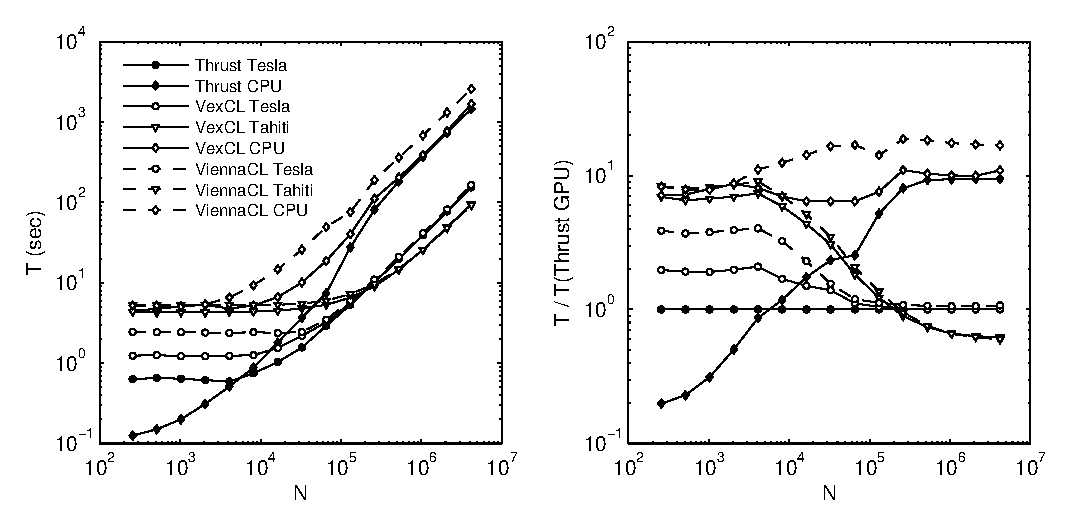
\includegraphics[width=\textwidth]{data/damped_oscillator/perfcmp}
%     \end{center}
%     \caption{Damped harmonic oscillator ensemble results.}
%     \label{fig:damped:perf}
% \end{figure}

\begin{figure}
    \begin{center}
        \subfigure[
        NVIDIA Tesla C2070.
        ]{\label{fig:damped:perf:tesla}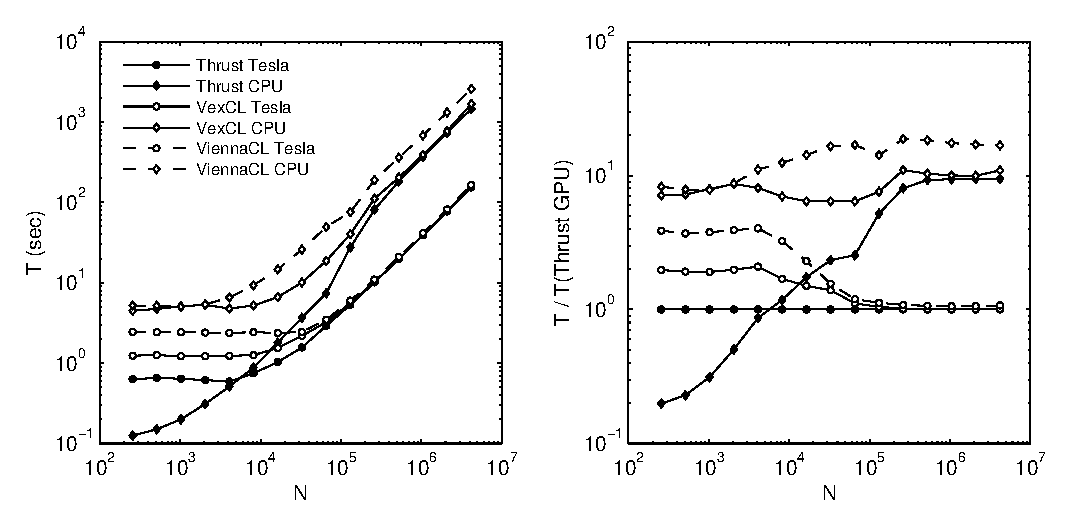
\includegraphics[width=\textwidth]{data/damped_oscillator/perfcmp_tesla}}
        \subfigure[
        AMD Radeon HD 7970 (Tahiti).
        ]{\label{fig:damped:perf:tahiti}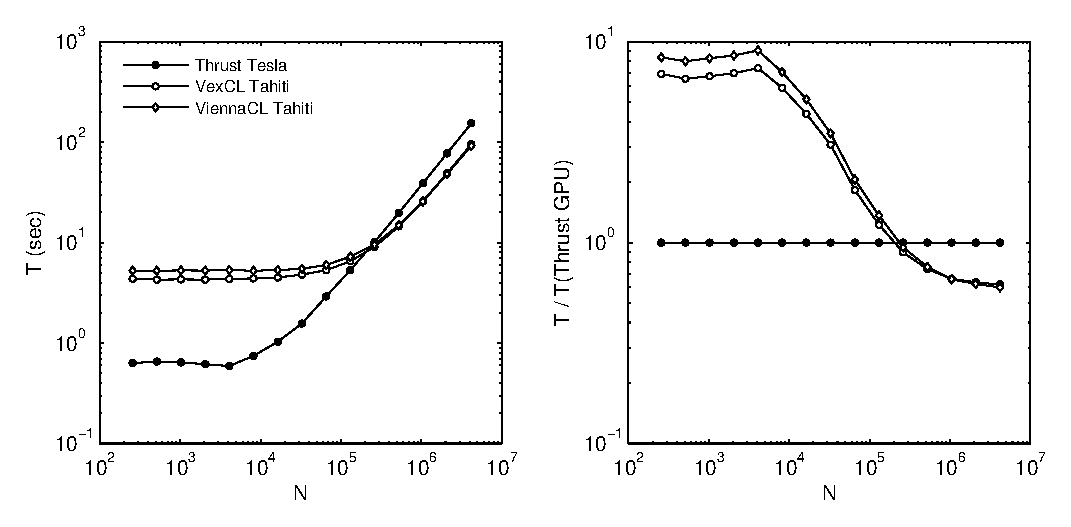
\includegraphics[width=\textwidth]{data/damped_oscillator/perfcmp_tahiti}}
    \end{center}
    \caption{Damped harmonic oscillator ensemble results.}
    \label{fig:damped:perf}
\end{figure}

%\begin{figure}
%    \begin{center}
%        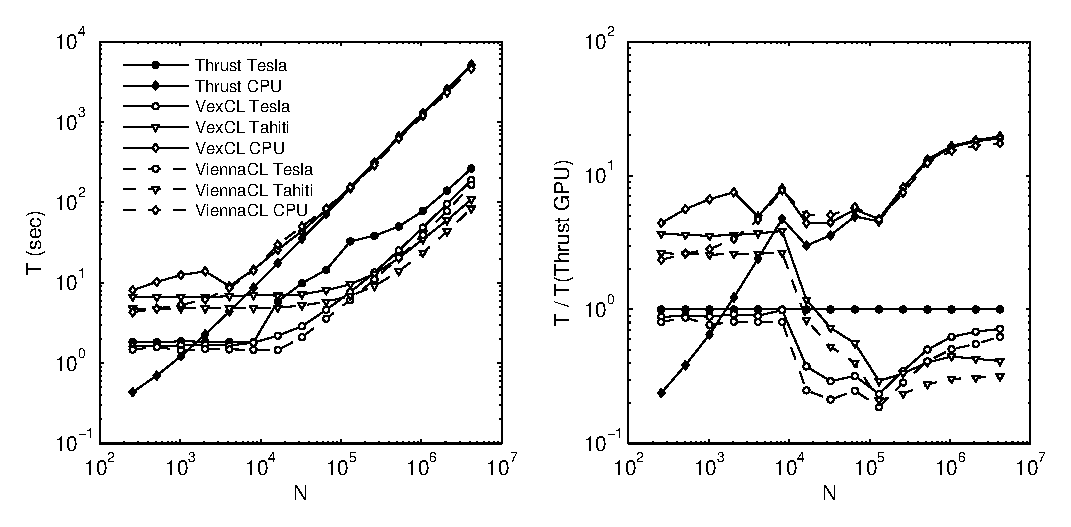
\includegraphics[width=\textwidth]{data/phase_oscillator_chain/perfcmp}
%    \end{center}
%    \caption{Coupled phase oscillator chain results.}
%    \label{fig:phase:perf}
%\end{figure}

\begin{figure}
    \begin{center}
        \subfigure[
        NVIDIA Tesla C2070.
        ]{\label{fig:phase:perf:tesla}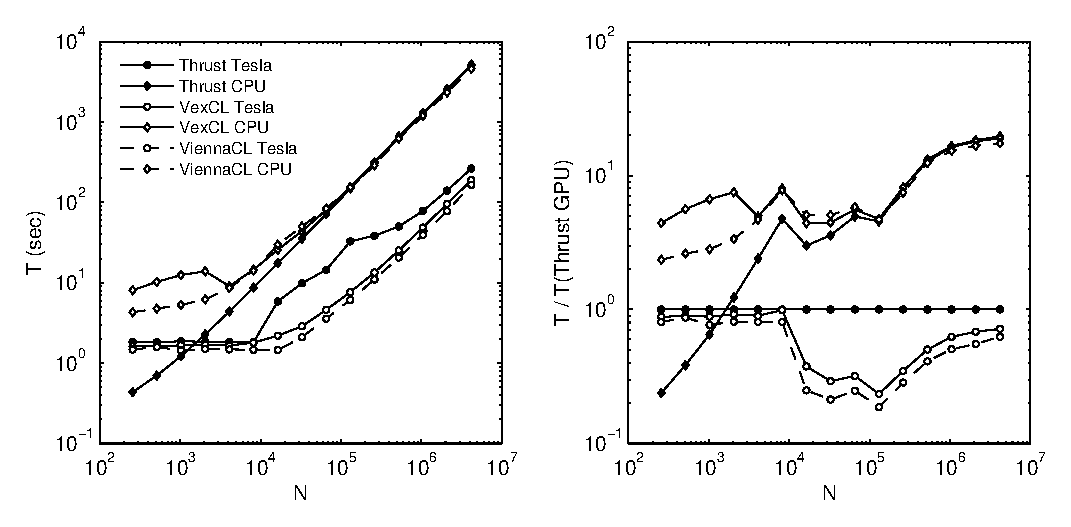
\includegraphics[width=\textwidth]{data/phase_oscillator_chain/perfcmp_tesla}}
        \subfigure[
        AMD Radeon HD 7970 (Tahiti).
        ]{\label{fig:phase:perf:tahiti}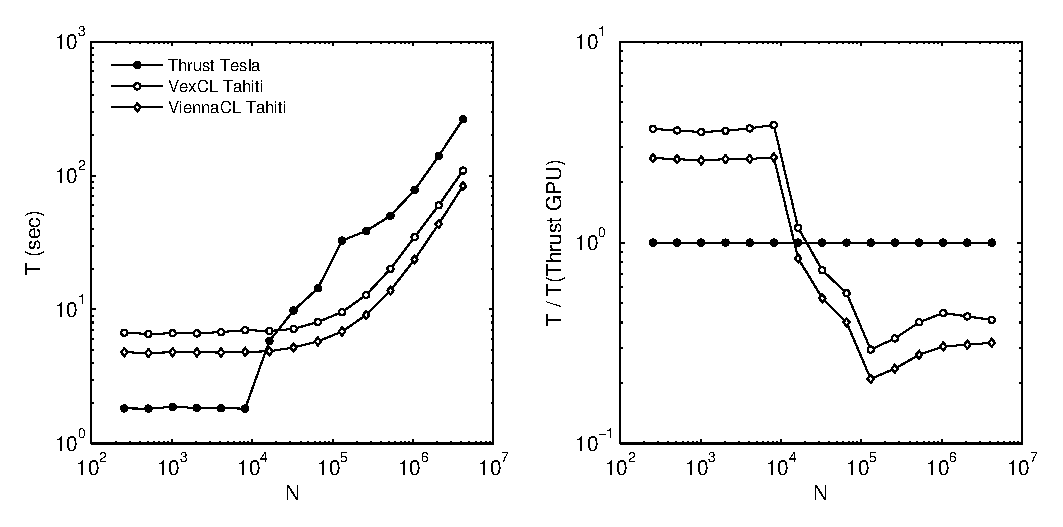
\includegraphics[width=\textwidth]{data/phase_oscillator_chain/perfcmp_tahiti}}
    \end{center}
    \caption{Coupled phase oscillator chain results.}
    \label{fig:phase:perf}
\end{figure}

%\begin{figure}
%    \begin{center}
%        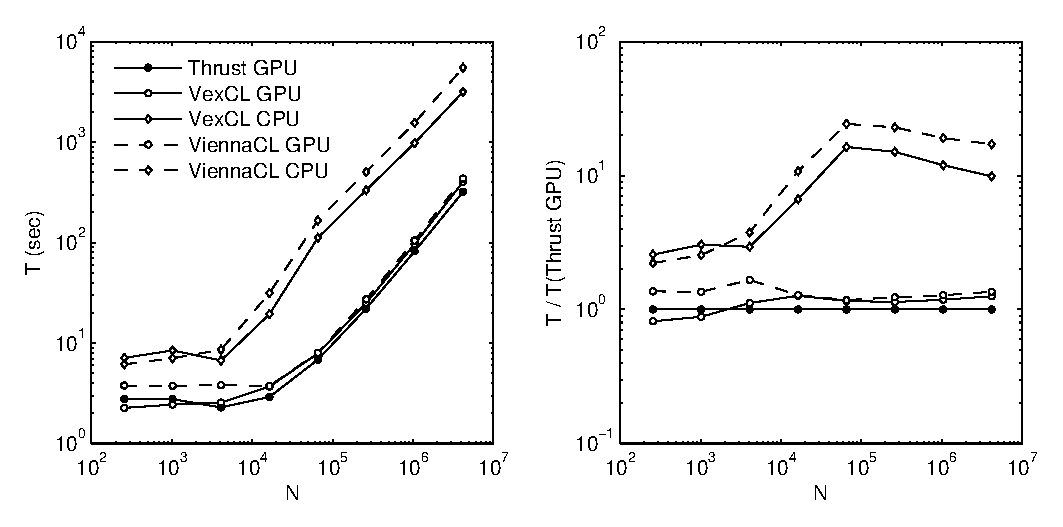
\includegraphics[width=\textwidth]{data/disordered_ham_lattice/perfcmp}
%    \end{center}
%    \caption{Disordered Hamiltonian lattice results.}
%    \label{fig:lattice:perf}
%\end{figure}

\begin{figure}
    \begin{center}
        \subfigure[
        NVIDIA Tesla C2070.
        ]{\label{fig:lattice:perf:tesla}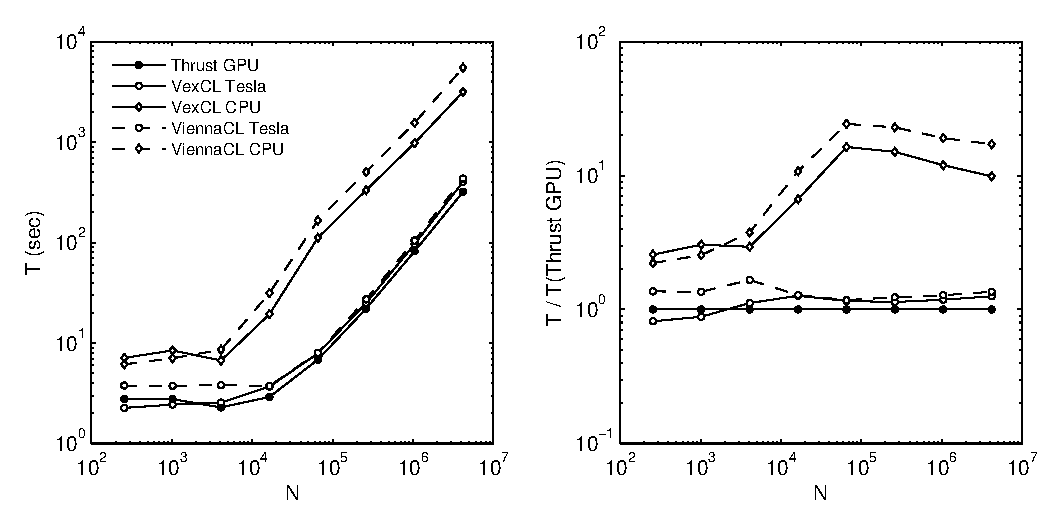
\includegraphics[width=\textwidth]{data/disordered_ham_lattice/perfcmp_tesla}}
        \subfigure[
        AMD Radeon HD 7970 (Tahiti).
        ]{\label{fig:lattice:perf:tahiti}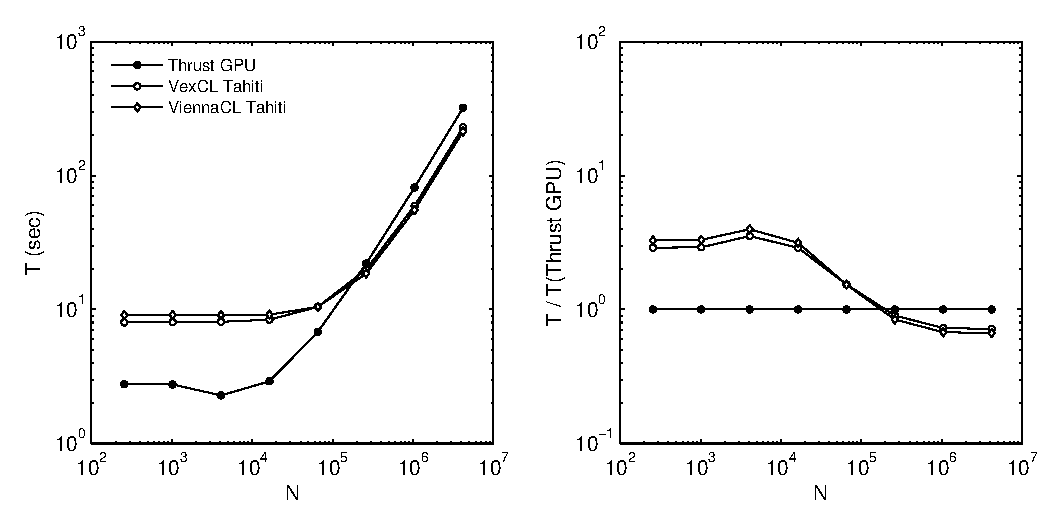
\includegraphics[width=\textwidth]{data/disordered_ham_lattice/perfcmp_tahiti}}
    \end{center}
    \caption{Disordered Hamiltonian lattice results.}
    \label{fig:lattice:perf}
\end{figure}


%\begin{figure}
%    \begin{center}
%        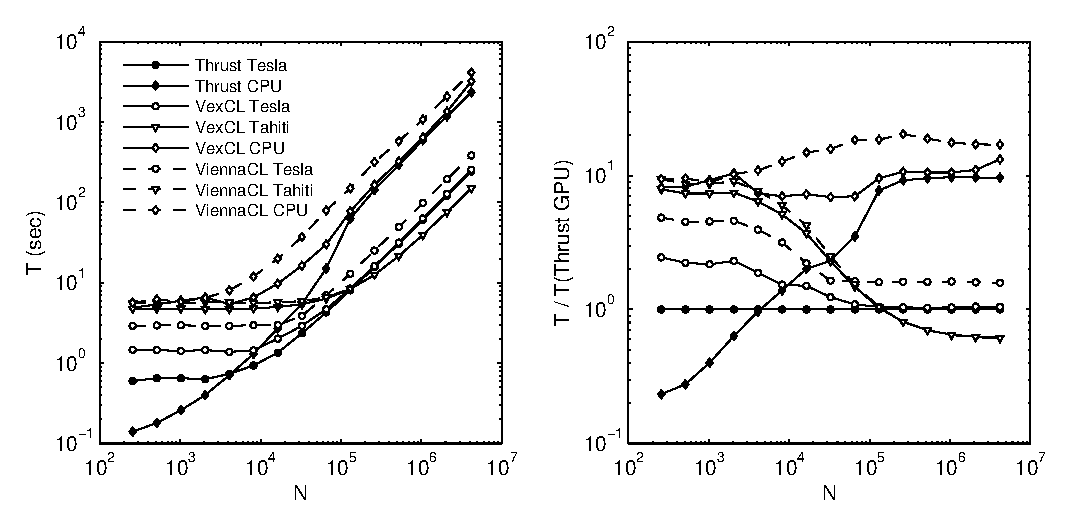
\includegraphics[width=\textwidth]{data/lorenz_ensemble/perfcmp}
%    \end{center}
%    \caption{Lorenz attractor ensemble results.}
%    \label{fig:lorenz:perf}
%\end{figure}

% \begin{figure}
%     \begin{center}
%       \subfigure[
%       NVIDIA Tesla C2070.
%       ]{\label{fig:lorenz:perf:tesla}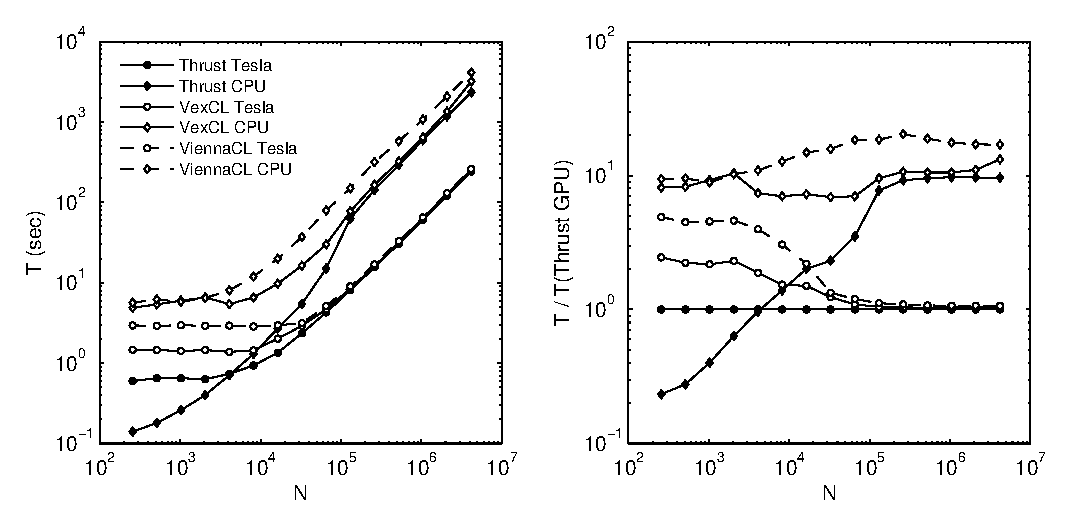
\includegraphics[width=\textwidth]{data/lorenz_ensemble/perfcmp_tesla}}
%       \subfigure[
%       AMD Radeon HD 7970 (Tahiti).
%       ]{\label{fig:lorenz:perf:tahiti}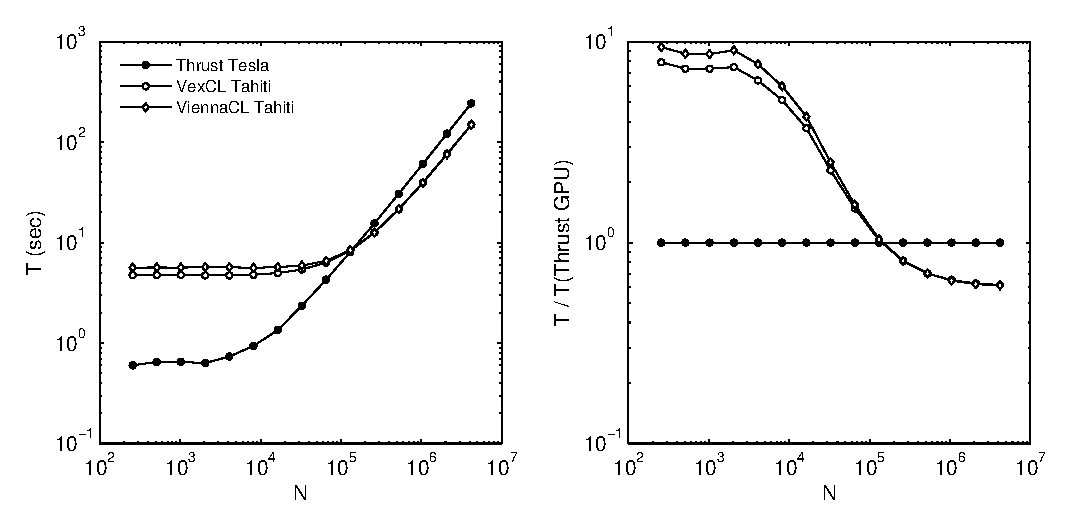
\includegraphics[width=\textwidth]{data/lorenz_ensemble/perfcmp_tahiti}}
%     \end{center}
%     \caption{Lorenz attractor ensemble results.}
%     \label{fig:lorenz:perf}
% \end{figure}

In general, all our experiments show up to $10\times$ to $20\times$ acceleration
when run on a GPU as compared to the CPU path. This is the expected acceleration
rate for the memory bandwidth bound examples that we looked at. However, both CUDA and OpenCL
programs show considerable overhead for the smaller problem sizes,
thus requiring problems of sizes between $10^3$ and $10^5$ to see any significant acceleration on
a GPU at all. The overhead for OpenCL libraries is larger than that of CUDA programs,
which is mostly due to the additional kernel management logic required by the OpenCL runtime.

Performance-wise, all of the considered libraries are close to each other when
run on a GPU.  Thrust performs slightly better in most cases except for the phase oscillator chain example,
where the permutation iterators require the use of an auxilary index vector.
VexCL and ViennaCL are in general slower than Thrust by a few percent, which is usually negligible in practice.
Apparently, the CUSPARSE implementation of the sparse matrix-vector product is more efficient than that of the OpenCL
libraries, since VexCL and ViennaCL are slower than Thrust/CUSPARSE combination
by about 30 percent for the disordered Hamiltonian lattice experiment. Both
OpenCL libraries show very similar results on a GPU. ViennaCL is about 15 percent faster for
phase oscillator chain example due to the use of a hand-written kernel.
Conversely, the overhead of using high-level libraries is negligible compared to the effort spent in getting familiar with the details of CUDA or OpenCL.
Thus, we have successfully countered productivity concerns for GPU computing raised in the past \cite{bordawekar:gpu-productivity}.

If we look at the performance of the experiments on the CPU, performance
differences between the libraries are more pronounced. Thrust outperforms
VexCL on larger problems by 15 to 40 percent, except for the chain of coupled phase
oscillators example, where VexCL is faster by about 5 percent.
The performance of ViennaCL on the CPU is poor and about 75 percent below that of Thrust and between 30 and 70 percent below that of VexCL.
The only exception is again the phase oscillator test, where ViennaCL outperforms other libraries.

\begin{table}
 \centering
    \caption{Absolute run times (sec) for the largest problem size.}
    \label{tab:abstimes}
    \begin{tabular}{|lc|rrr|}
        \hline
        & & \em Damped      & \em Coupled       & \em Disordered  \\ %  & \em Lorenz    \\
        & & \em harmonic    & \em phase         & \em Hamiltonian \\ %  & \em attractor \\
        & & \em oscillators & \em oscillators   & \em lattice     \\ %  & \em ensemble  \\
        \hline
        \em Thrust   &\em Tesla & 153.53 & 263.99 & 319.54 \\ %  & 242.75 \\
        \em VexCL    &\em Tesla & 154.76 & 189.38 & 401.31 \\ %  & 255.06 \\
        \em ViennaCL &\em Tesla & 164.52 & 165.21 & 433.24 \\ %  & 259.82 \\
        \hline
        \em VexCL    &\em Tahiti &  94.97 & 108.83 & 228.93 \\ %  & 149.20 \\
        \em ViennaCL &\em Tahiti &  91.73 &  83.61 & 213.22 \\ %  & 148.62 \\
        \hline
        \em Thrust   &\em CPU   & 1~454.81 & 5~172.84 &      N/A \\ %  & 2~339.33 \\
        \em VexCL    &\em CPU   & 1~678.26 & 5~015.02 & 3~152.92 \\ %  & 3~206.17 \\
        \em ViennaCL &\em CPU   & 2~574.70 & 4~605.93 & 5~485.99 \\ %  & 4~127.98 \\
        \hline
    \end{tabular}
\end{table}


The difference between Thrust and the OpenCL libraries can be explained by the fact
that Thrust uses OpenMP backend when run on a CPU. Thus, it does not have any
overhead such as OpenCL initialization and kernel compilation.  The gap
between OpenCL libraries may be attributed to the different workgroup sizes
used in their kernels and the fact that VexCL generates slightly different
kernels when run on a CPU device. Moreover, both of the libraries are primarily
aimed at GPU performance and do not use CPU-specific optimizations, such as
employing OpenCL vector data types that facilitate use of SSE instructions.
Still, the overhead of OpenCL for small problem sizes is tremendous, if not embarrasing,
hence OpenCL cannot be considered to be a competitive CPU programming model for a large area of applications in its present state. % [KR]: Please let me know whether you agree with this sentence. It is a rather bold statement, yet the only reasonable one when looking at the benchmark results.

Finally, results for multi-GPU usage as provided by VexCL in a transparent way are considered.
\figref{fig:scaling} shows scaling results for up to three Tesla C2070 GPUs.
It can be seen that a notable speed-up of several GPUs over a single GPU is only obtained for problem sizes
larger than $10^6$.
\figref{fig:scaling:damped} also shows scaling results for the system with three Tahiti GPUs. % [KR]: What about results for Tahiti? Either include results for all examples, or for none.
It seems that AMD OpenCL
implementation does not work very well with multiple GPUs employed. Still,
combined memory of several GPUs allows to solve proportionally larger problems
on the same system.

% [KR]:
\begin{figure}
    \begin{center}
        \subfigure[
        Damped harmonic oscillator ensemble.
        ]{\label{fig:scaling:damped}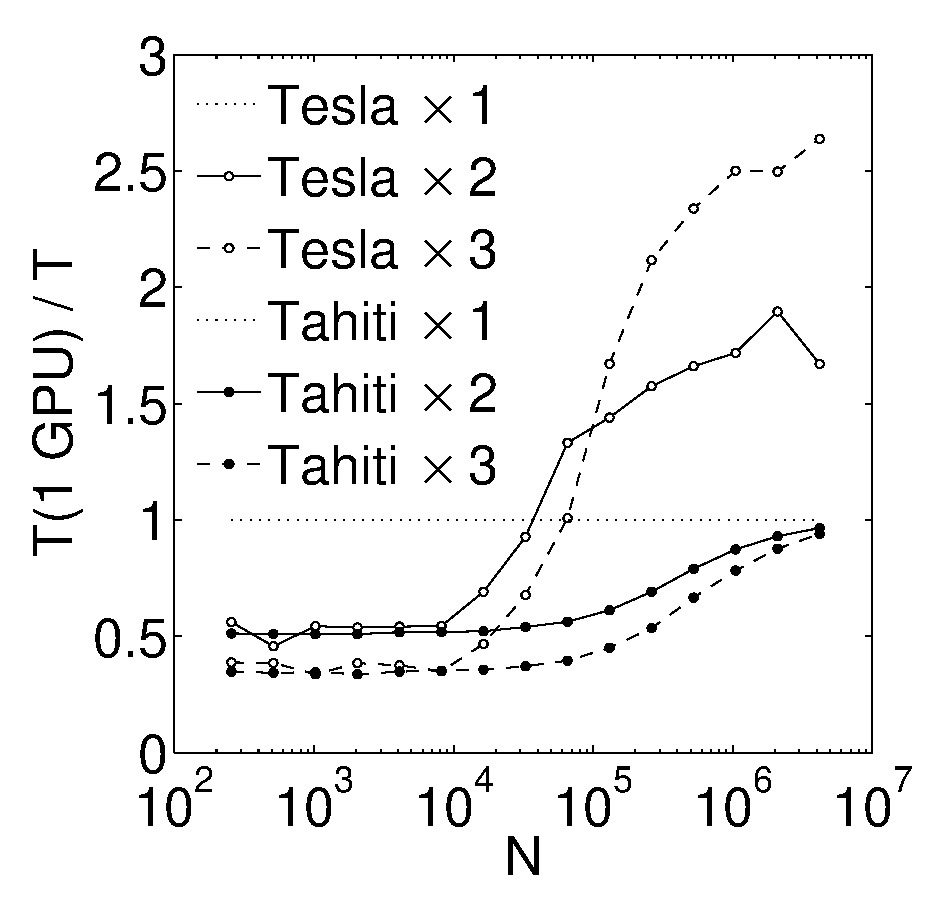
\includegraphics[width=0.32\textwidth]{data/damped_oscillator/scaling}}$\;$
        \subfigure[
        Coupled phase oscillator chain.
        ]{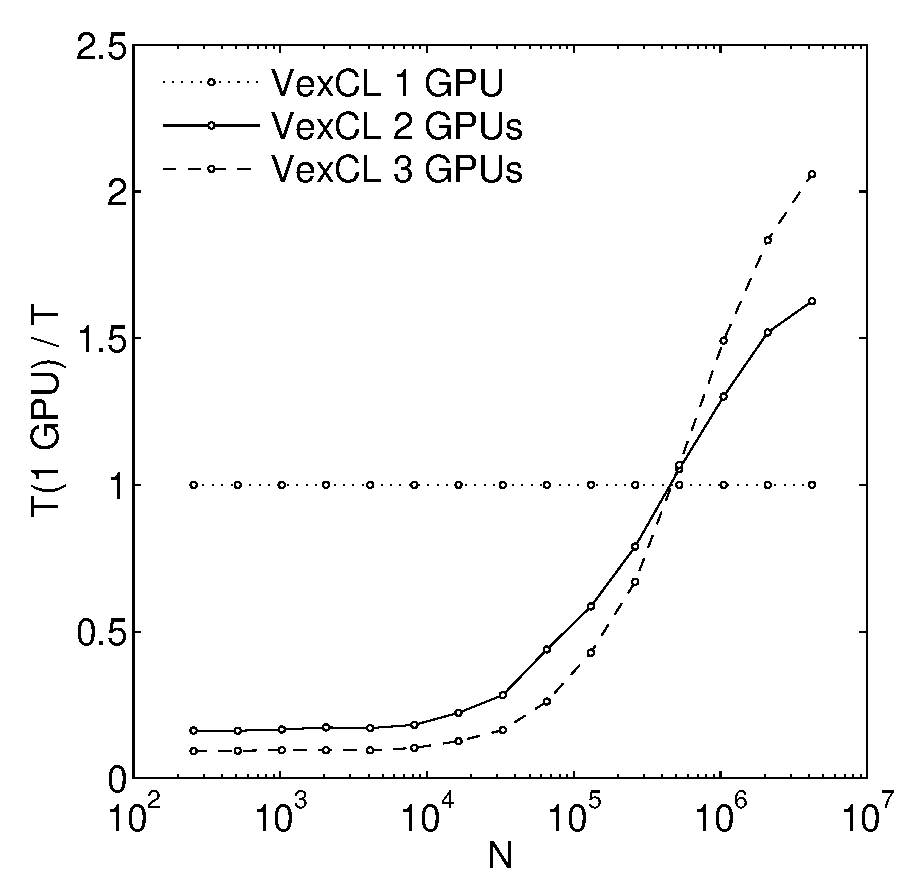
\includegraphics[width=0.32\textwidth]{data/phase_oscillator_chain/scaling}}$\;$
        \subfigure[
        Disordered Hamiltonian lattice.
        ]{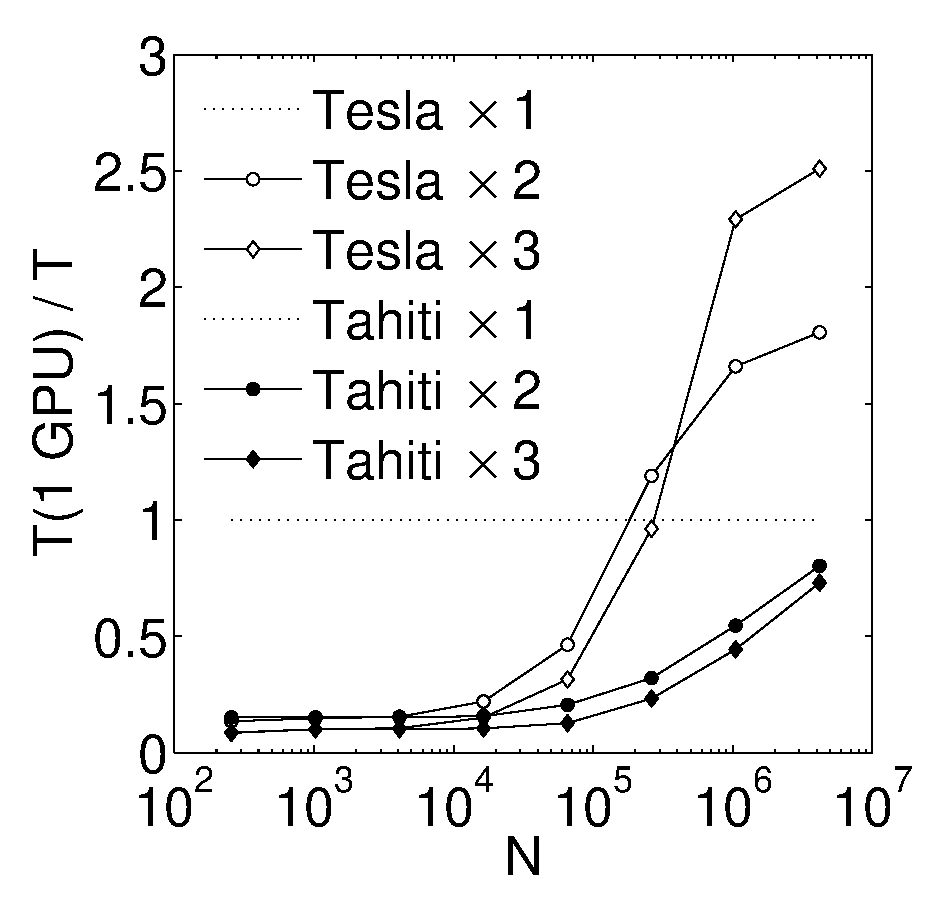
\includegraphics[width=0.32\textwidth]{data/disordered_ham_lattice/scaling}}
        %\subfigure[
        %Lorenz attractor ensemble.
        %]{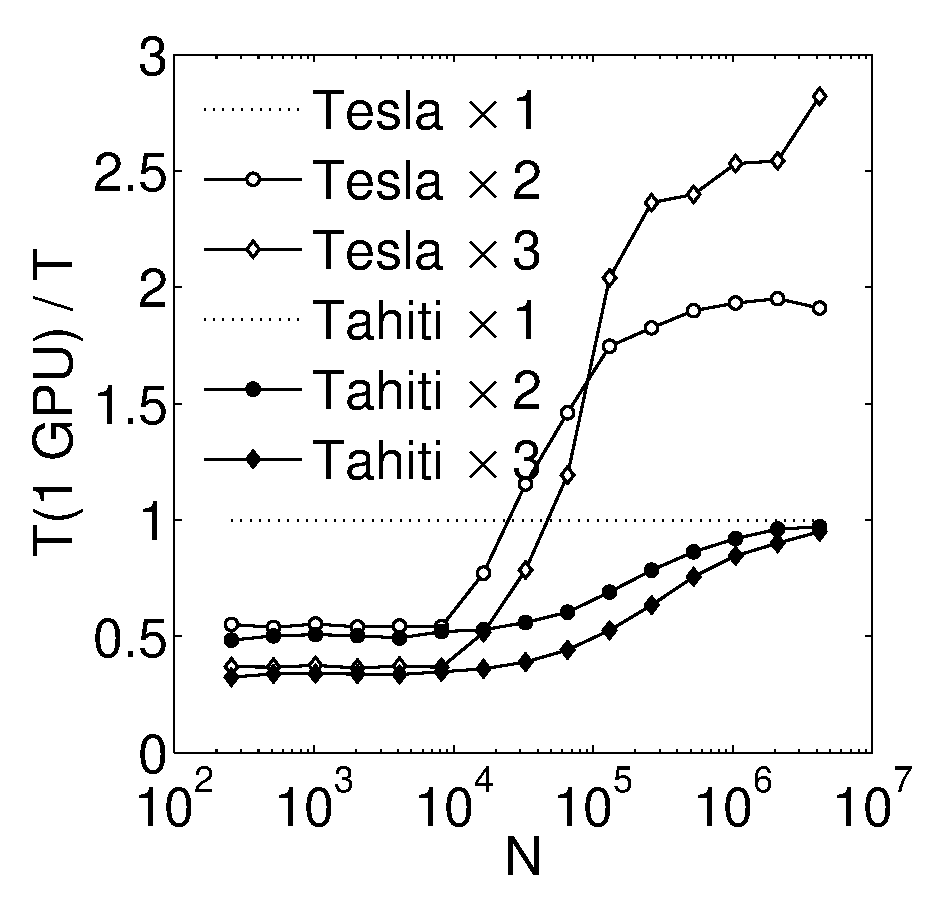
\includegraphics[width=0.45\textwidth]{data/lorenz_ensemble/scaling}}
    \end{center}
    \caption{VexCL scaling with multigpu computation.}
    \label{fig:scaling}
\end{figure}


% [KR]: I integrated the following paragraph in the conclusions. Please double-check.
%
%VexCL was the only library that managed to stay at high level and did not need
%help of third party libraries in all of our examples. ViennaCL lacks some
%elementwise vector operations and stencil convolution operation, so we had to
%provide hand-written kernels for those; Thrust version of coupled phase
%oscillator chain example needed help of CUSPARSE library for implemetation of
%sparse matrix~-- vector product.









%
% CONCLUSION
%
\section{Conclusion}

Performance-wise, there is almost no difference between various platforms and
libraries when those are run on the same hardware. As we have shown, various
computational problems may be solved effectively in terms of both human and
machine time with the help of modern high-level libraries.  There are some
differences in the programming interfaces of the libraries which may be crucial
for ones specific application.

The focus of Thrust is more on providing low-level primitives with an interface
very close to the C++ STL library.
Special purpose functionality is available via separate libraries such as CUSPARSE
and can be integrated without a lot of effort.
The OpenCL libraries we looked at demonstrated that they are able to
provide more convenient interface for a scientific programmer than a direct
implementation in CUDA or OpenCL.
VexCL has a richer set of elementwise vector operations and allows for the
shortest implementations in the context of ODEs considered in this work.
ViennaCL required a few additional lines of code including small custom OpenCL kernels for our examples.
Still, this extra effort is acceptable considering that the library's focus is on sparse linear systems solvers,
which are, however, beyond the scope of this paper.

Regarding a comparison of CUDA versus OpenCL, the main difference observed in this work is the wider range of hardware supported.
Although performance obtained via CUDA is a few percent better than that of OpenCL on the overall,
the differences are mostly too small in order to make decision in favor of CUDA based on performance only.
Moreover, the slight performance advantage of CUDA can still turn into a disadvantage when taking the larger set of hardware supporting OpenCL into consideration.


Another aspect that has not been studied in this work is the ability to generate kernels
optimized for the problem at hand at runtime. This allows, for example, to generate
optimized kernels for a certain set of parameters supplied, eliminating any otherwise spurious reads from global memory.
An in-depth study of such an approach is, however, left for future work.

% [DD]: OpenCL libraries showed excelent functional portability but not so good
% performance portability.

% [DD]: Some words about odeint generality that allowed us to run the set of
% experiments.



\section{Acknowledgments}

This work has been partially supported by the Russian Foundation for Basic
Research (RFBR) grant No 12-07-0007 and the Austrian Science Fund (FWF), grant P23598.
We also would like to thank Gradient JSC\footnote{ \href{
http://www.gradient-geo.com/en }{ http://www.gradient-geo.com/en } } for the
kindly provided AMD hardware.


\bibliographystyle{siam}
\bibliography{ref}

\end{document}
% vim: set et
